\begin{figure}
\centering
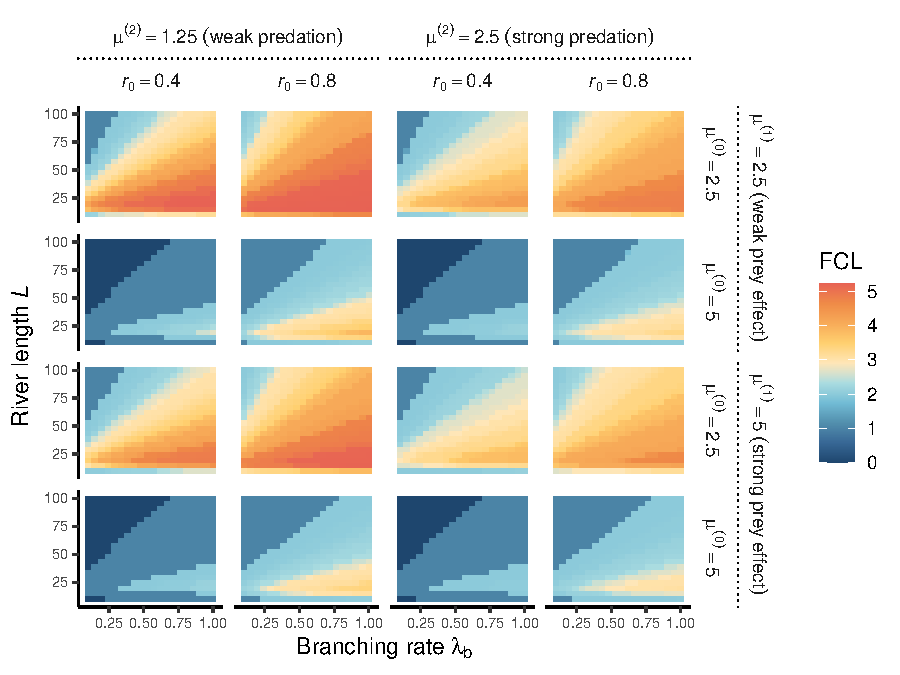
\includegraphics{../data_fmt/fig_theo_rho025_g75_theta025.pdf}
\caption{\label{fig:fig-num1}Numerical prediction with low propagule
\(g_0 = 75\), low synchrony \(\rho = 0.25\), and weak omnivory
\(\theta = 0.25\). Heatmaps of FCL are expressed as a function of
ecosystem size (river length, \(L\)) and complexity (branching rate,
\(\lambda_b\)), with rows and columns displaying different combinations
of resource supply (\(r_0\)), disturbance regime (\(\mu^{(0)}\)), prey
effect (\(\mu^{(1)}\)), and predation effect (\(\mu^{(2)}\)). Each cell
represents the average FCL of five food webs. Additional parameter
values are: habitat density \(h=2.5\), dispersal capability
\(\delta_0=0.5\), and scaling exponent \(\psi=0.5\).}
\end{figure}

\newpage

\begin{figure}
\centering
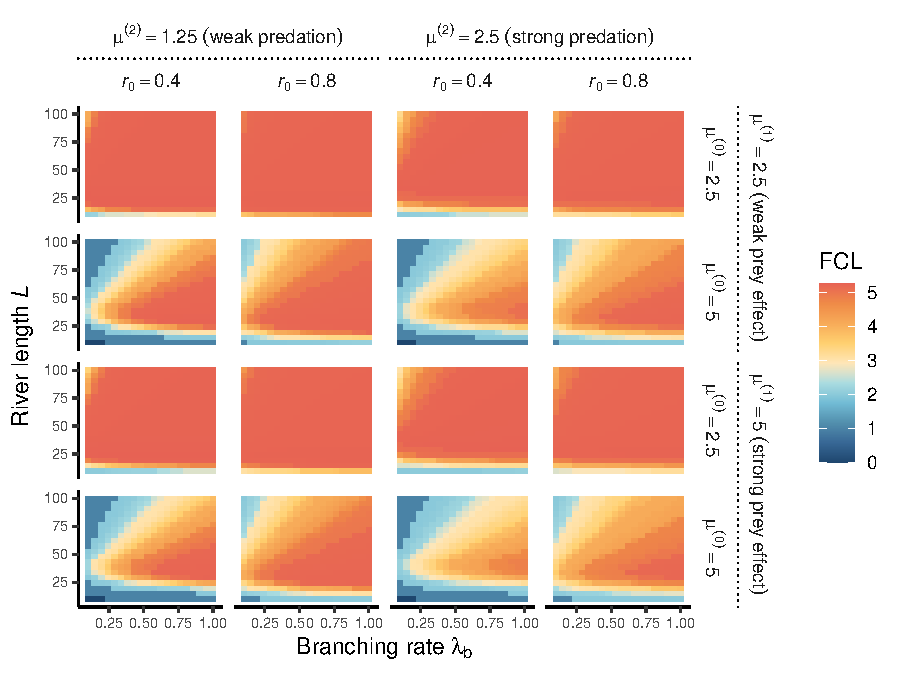
\includegraphics{../data_fmt/fig_theo_rho025_g150_theta025.pdf}
\caption{\label{fig:fig-num2}Numerical prediction with high propagule
\(g_0 = 150\), low synchrony \(\rho = 0.25\), and weak omnivory
\(\theta = 0.25\). Heatmaps of FCL are expressed as a function of
ecosystem size (river length, \(L\)) and complexity (branching rate,
\(\lambda_b\)), with rows and columns displaying different combinations
of resource supply (\(r_0\)), disturbance regime (\(\mu^{(0)}\)), prey
effect (\(\mu^{(1)}\)), and predation effect (\(\mu^{(2)}\)). Each cell
represents the average FCL of five food webs. Additional parameter
values are: habitat density \(h=2.5\), dispersal capability
\(\delta_0=0.5\), and scaling exponent \(\psi=0.5\).}
\end{figure}

\newpage

\begin{figure}
\centering
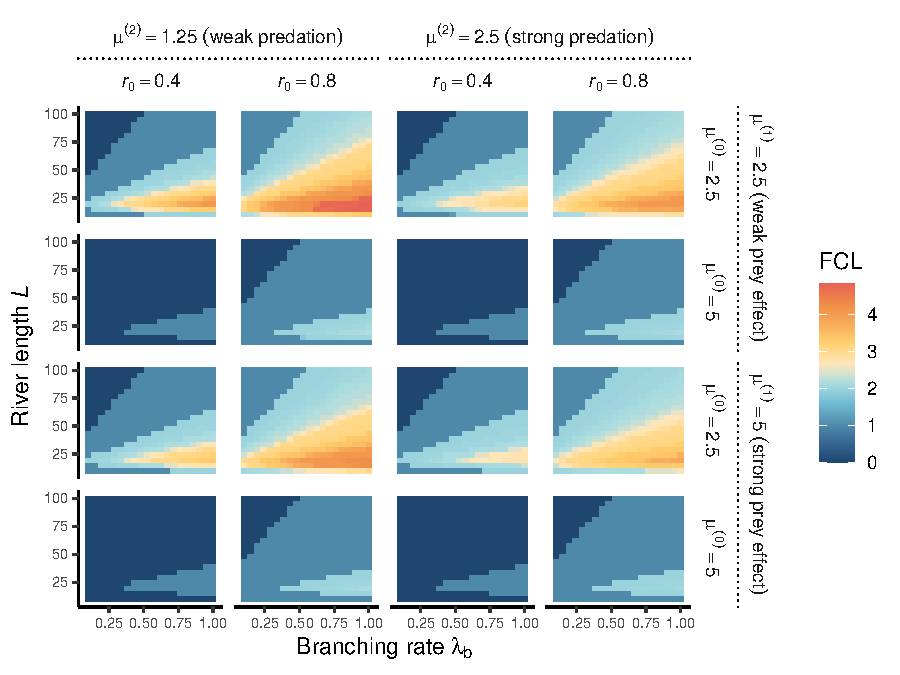
\includegraphics{../data_fmt/fig_theo_rho05_g75_theta025.pdf}
\caption{\label{fig:fig-num3}Numerical prediction with low propagule
\(g_0 = 75\), high synchrony \(\rho = 0.5\), and weak omnivory
\(\theta = 0.25\). Heatmaps of FCL are expressed as a function of
ecosystem size (river length, \(L\)) and complexity (branching rate,
\(\lambda_b\)), with rows and columns displaying different combinations
of resource supply (\(r_0\)), disturbance regime (\(\mu^{(0)}\)), prey
effect (\(\mu^{(1)}\)), and predation effect (\(\mu^{(2)}\)). Each cell
represents the average FCL of five food webs. Additional parameter
values are: habitat density \(h=2.5\), dispersal capability
\(\delta_0=0.5\), and scaling exponent \(\psi=0.5\).}
\end{figure}

\newpage

\begin{figure}
\centering
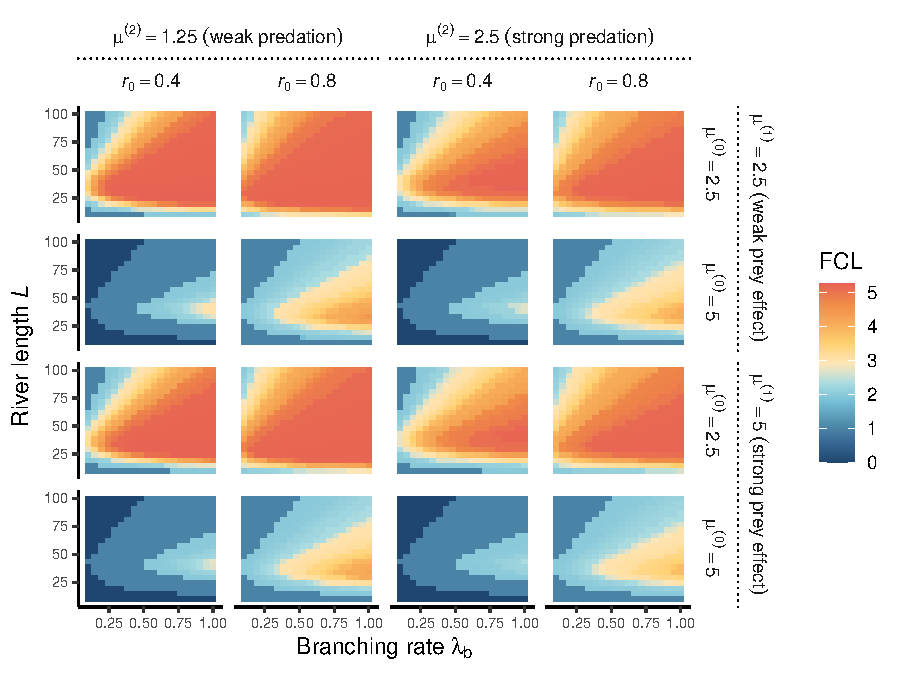
\includegraphics{../data_fmt/fig_theo_rho05_g150_theta025.pdf}
\caption{\label{fig:fig-num4}Numerical prediction with high propagule
\(g_0 = 150\), high synchrony \(\rho = 0.5\), and weak omnivory
\(\theta = 0.25\). Heatmaps of FCL are expressed as a function of
ecosystem size (river length, \(L\)) and complexity (branching rate,
\(\lambda_b\)), with rows and columns displaying different combinations
of resource supply (\(r_0\)), disturbance regime (\(\mu^{(0)}\)), prey
effect (\(\mu^{(1)}\)), and predation effect (\(\mu^{(2)}\)). Each cell
represents the average FCL of five food webs. Additional parameter
values are: habitat density \(h=2.5\), dispersal capability
\(\delta_0=0.5\), and scaling exponent \(\psi=0.5\).}
\end{figure}

\newpage

\begin{figure}
\centering
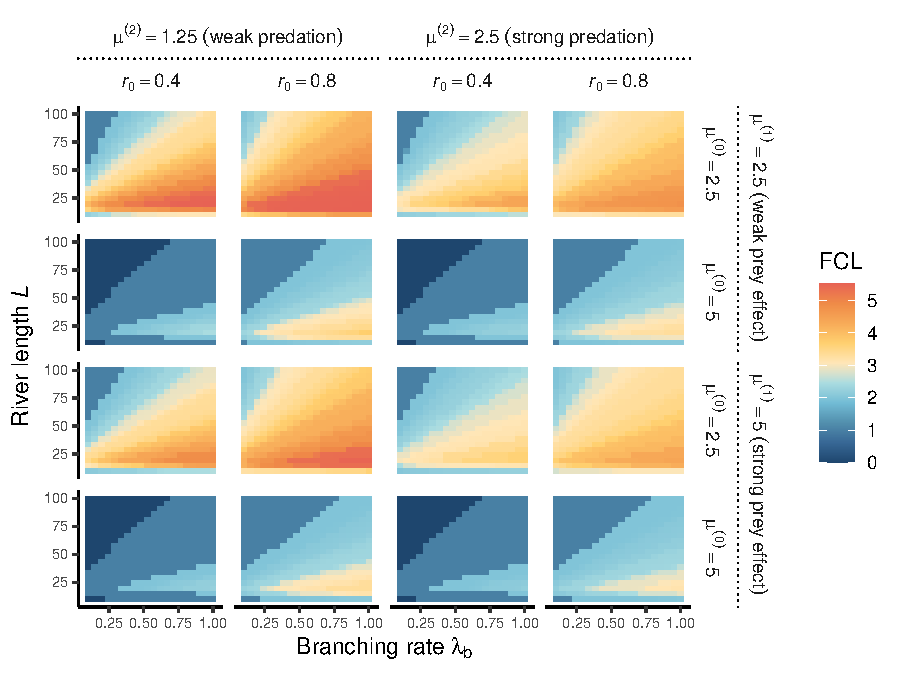
\includegraphics{../data_fmt/fig_theo_rho025_g75_theta05.pdf}
\caption{\label{fig:fig-num5}Numerical prediction with low propagule
\(g_0 = 75\), low synchrony \(\rho = 0.25\), and strong omnivory
\(\theta = 0.5\).Heatmaps of FCL are expressed as a function of
ecosystem size (river length, \(L\)) and complexity (branching rate,
\(\lambda_b\)), with rows and columns displaying different combinations
of resource supply (\(r_0\)), disturbance regime (\(\mu^{(0)}\)), prey
effect (\(\mu^{(1)}\)), and predation effect (\(\mu^{(2)}\)). Each cell
represents the average FCL of five food webs. Additional parameter
values are: habitat density \(h=2.5\), dispersal capability
\(\delta_0=0.5\), and scaling exponent \(\psi=0.5\).}
\end{figure}

\newpage

\begin{figure}
\centering
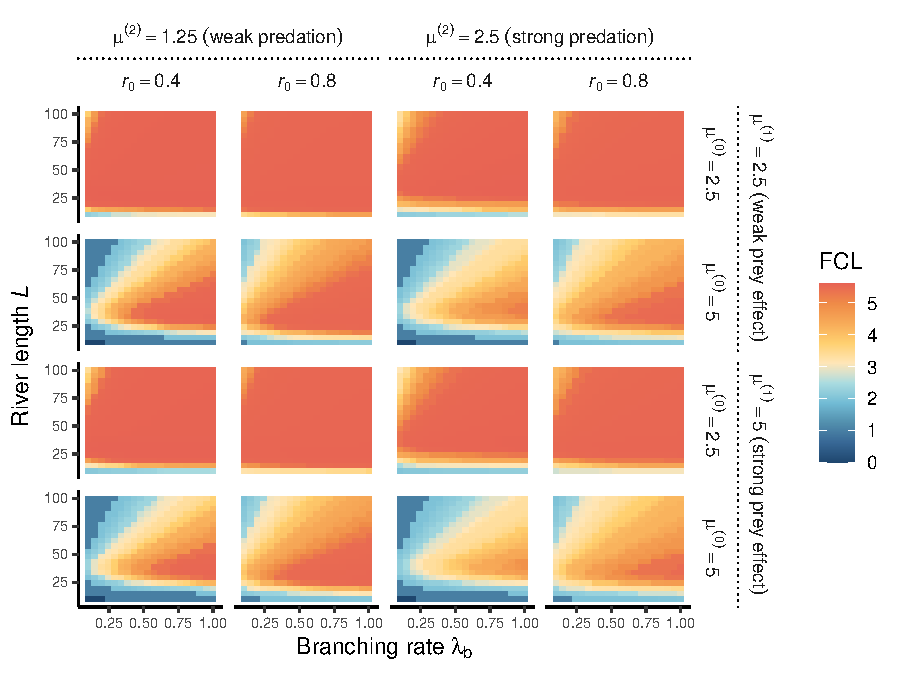
\includegraphics{../data_fmt/fig_theo_rho025_g150_theta05.pdf}
\caption{\label{fig:fig-num6}Numerical prediction with high propagule
\(g_0 = 150\), low synchrony \(\rho = 0.25\), and strong omnivory
\(\theta = 0.5\).Heatmaps of FCL are expressed as a function of
ecosystem size (river length, \(L\)) and complexity (branching rate,
\(\lambda_b\)), with rows and columns displaying different combinations
of resource supply (\(r_0\)), disturbance regime (\(\mu^{(0)}\)), prey
effect (\(\mu^{(1)}\)), and predation effect (\(\mu^{(2)}\)). Each cell
represents the average FCL of five food webs. Additional parameter
values are: habitat density \(h=2.5\), dispersal capability
\(\delta_0=0.5\), and scaling exponent \(\psi=0.5\).}
\end{figure}

\newpage

\begin{figure}
\centering
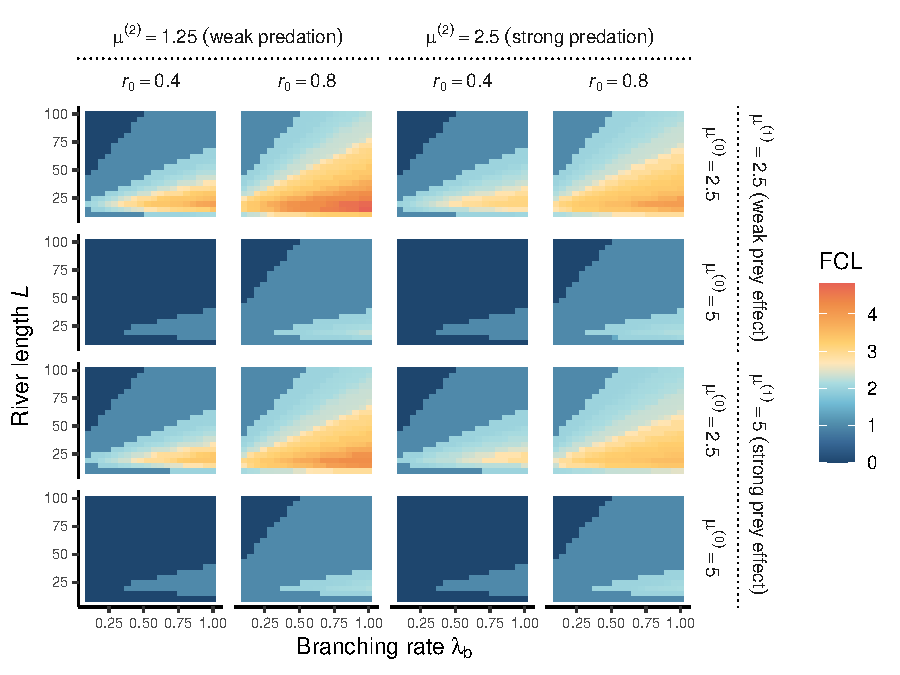
\includegraphics{../data_fmt/fig_theo_rho05_g75_theta05.pdf}
\caption{\label{fig:fig-num7}Numerical prediction with low propagule
\(g_0 = 75\), high synchrony \(\rho = 0.5\), and strong omnivory
\(\theta = 0.5\).Heatmaps of FCL are expressed as a function of
ecosystem size (river length, \(L\)) and complexity (branching rate,
\(\lambda_b\)), with rows and columns displaying different combinations
of resource supply (\(r_0\)), disturbance regime (\(\mu^{(0)}\)), prey
effect (\(\mu^{(1)}\)), and predation effect (\(\mu^{(2)}\)). Each cell
represents the average FCL of five food webs. Additional parameter
values are: habitat density \(h=2.5\), dispersal capability
\(\delta_0=0.5\), and scaling exponent \(\psi=0.5\).}
\end{figure}

\newpage

\begin{figure}
\centering
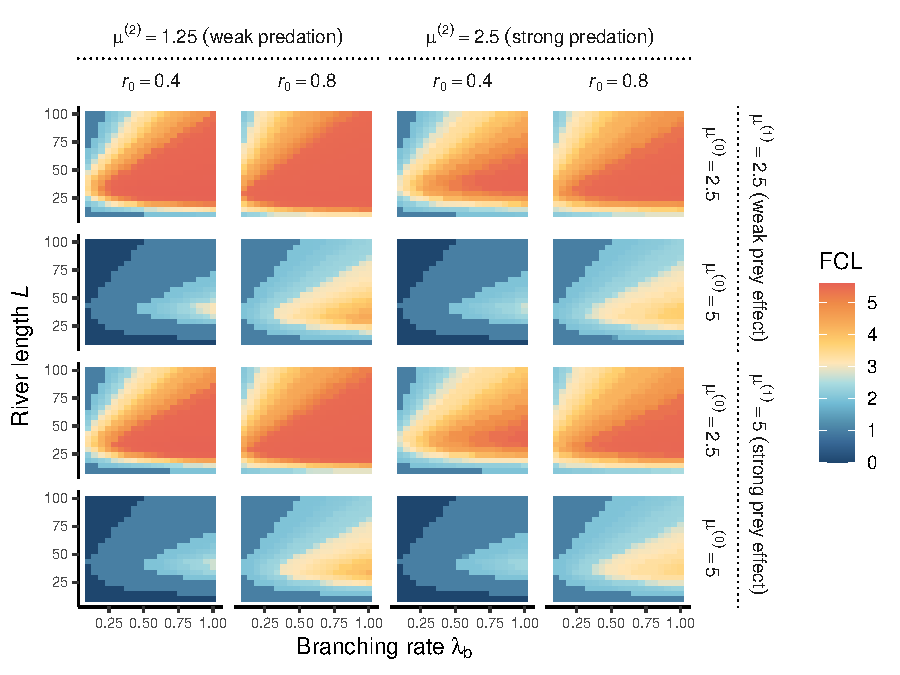
\includegraphics{../data_fmt/fig_theo_rho05_g150_theta05.pdf}
\caption{\label{fig:fig-num8}Numerical prediction with high propagule
\(g_0 = 150\), high synchrony \(\rho = 0.5\), and strong omnivory
\(\theta = 0.5\).Heatmaps of FCL are expressed as a function of
ecosystem size (river length, \(L\)) and complexity (branching rate,
\(\lambda_b\)), with rows and columns displaying different combinations
of resource supply (\(r_0\)), disturbance regime (\(\mu^{(0)}\)), prey
effect (\(\mu^{(1)}\)), and predation effect (\(\mu^{(2)}\)). Each cell
represents the average FCL of five food webs. Additional parameter
values are: habitat density \(h=2.5\), dispersal capability
\(\delta_0=0.5\), and scaling exponent \(\psi=0.5\).}
\end{figure}

\newpage
